\documentclass[a4paper,12pt]{article}

\usepackage[T1]{fontenc}
\usepackage[utf8]{inputenc}
\usepackage[top=2cm, bottom=3cm, left=1.5cm, right=1.5cm]{geometry}
\usepackage{fancyhdr}
\usepackage[pdftex]{graphicx}
\usepackage{graphics}
\usepackage{latexsym}
\usepackage{amsmath,amsfonts,amssymb}
\usepackage{tikz}
% \usepackage{placeins}
% \usepackage[french, figure, boxed, longend]{algorithm2e}
\usepackage[francais,english]{babel}


% En-t�tes et pieds de page
\pagestyle{fancy}
\headheight 35pt
\lhead{\textbf{\begin{small}Rapport Projet 2008-2009\end{small}}}
\chead{\textsc{\begin{large}Etude de la topologie de l'Internet\end{large}}}
\rhead{\textbf{\begin{small}\end{small}}}
\lfoot{2008}
\rfoot{\thepage}
\cfoot{}

\newcommand{\boost}{\textit{Boost}}

%opening
\title{}
\author{}

\begin{document}

\maketitle

\begin{abstract}

\end{abstract}

%TODOpour les définitions :
% clique / full-mesh
% Autonomous System AS
% graphe connexe
% centralit\'e

\newpage
\section{Visualisation de la topologie inter-domaine de l'Internet}

% \documentclass[a4paper,10pt]{article}

% \begin{document}

\subsection{Tomographie de l'Internet inter-domaine}

\subsubsection{Pr\'esentation d'Internet}

\par
Aujourd'hui, le r\'eseau le plus connu de part le monde est l'Internet. Il est le fruit combin\'e de la recherche militaire et de l'inter\^et que lui ont ensuite port\'e les universitaires.
\par
%TODO Déplacer en Accroche d'introduction doit pas être là ce truc... mais gg pala ça a la classe pour l'accroche.
Au d\'ebut utilis\'e pour relier entre eux les principaux sites militaires des \'Etats-Unis, puis les universit\'es, Internet relie aujourd'hui des millions de foyers de part le monde, mais que se cache-t-il r\'eellement derri\`ere cette appellation?
\par
%TODO Fin deplacer
Internet est en fait un r\'eseau de r\'eseaux. Des r\'eseaux ind\'ependants appartenant \`a des entreprises priv\'ees, des universit\'es, des op\'erateurs. Ces r\'eseaux ind\'ependants sont appel\'es syst\`emes autonomes AS. Chaque r\'eseau est connect\'e \`a plusieurs autres et lorsque deux ordinateurs appartenant \`a des AS diff\'erents souhaitent communiquer, leurs paquets de donn\'ees seront rout\'es \`a travers l'Internet en passant par plusieurs AS interm\'ediaires. Aucun des \'el\'ements ne connait la totalit\'e de la topologie du r\'eseau et les paquets sont dirig\'es suivant des r\`egles de routage locales.
\par
Lorsque l'on parle de repr\'esenter Internet sous forme de graphe, dans la pr\'esente \'etude, il s'agit en fait de repr\'esenter les liens entre les diff\'erents AS. Cependant, il est n\'ecessaire de connaitre la topologie inter-AS au pr\'ealable pour pouvoir la repr\'esenter.

\subsubsection{Origine des donn\'ees}
\par
Il existe diff\'erents outils pour connaitre les liens entre les diff\'erents AS. Comme indiqu\'e sur le site \textit{www.caida.org} il existe au moins trois outils pour obtenir la topologie inter-AS :
\begin{description}
 \item[traceroute : ] outil permettant de capturer les adresses IP des diff\'erents \'equipements r\'eseau sur un chemin entre une source et une destination en utilisant des paquets sonde UDP ou ICMP. La r\'esolution du num\'ero d'AS associ\'e \'a chaque adresse IP permet d'obtenir une carte inter-AS.
 \item[BGP : ] protocole de routage inter-domaine utilis\'e pour le routage entre les AS. Ses tables de routage contiennent des chemins d'AS, on peut ainsi avoir une idée des liens entre les diff\'erents AS.
 \item[WHOIS : ] collection de bases de donn\'ees contenant des informations utiles aux op\'erateurs. Malheureusement, ces bases de donn\'ees sont maintenues \`a la main et ne  sont donc pas toujours tr\`es fiables. La plus sûre est la RIPE WHOIS qui regroupe des informations collect\'ees par la RIPE (service d'information sur les R\'eseaux IP Europ\'eens).
\end{description}
\par
Nous utiliserons principalement la m\'ethode BGP en raison de sa fiabilit\'e.

\subsubsection{Internet IPv4 et IPv6}
\par
Aujourd'hui, un changement majeur qui est en train de s'op\'erer dans les r\'eseaux : le passage de l'IPv4 \`a l'IPv6. En effet, si IPv4 permet l'utilisation d'un peu plus de quatre milliards d'adresses ($2^{32}$), IPv6 permet quant \`a lui d'utiliser $2^{128}$ adresses diff\'erentes, ce qui permet de combler les nouveaux besoins.
\par
La mise en place progressive de l'IPv6 se traduit au sein des grands r\'eseaux par une cohabitation entre les deux syst\`emes. On peut ainsi trouver des informations pour cr\'eer le graphe de topologie pour l'internet IPv4 mais aussi pour l'internet IPv6.
\par
Au cours de notre projet, nous avons eu successivement acc\`es aux donn\'ees de l'IPv4 puis de l'IPv6.
% \end{document}


%\documentclass[a4paper,12pt]{article}

%\usepackage{graphics}
%\usepackage[pdftex]{graphicx}

%\begin{document}

\subsection{Topologie de l'Internet}
\par
Commme expliqu\'e pr\'ec\'edemment Internet n'est pas un seul est grand r\'eseau, il s'agit en fait de l'interconnection de plusieurs r\'eseaux ou syst\`emes autonomes (AS). Un syst\`eme autonome est un r\'eseau r\'egit par une administration et soumis \`a un ensemble de r\`egles de routage internes. Les AS sont reli\'es entre eux par diff\'erents types de liens. Ces liens peuvent \^etre :
\begin{description}
 \item[PEER] il s'agit d'un accord commercial \`a travers lequel les clients respectifs de deux AS peuvent communiquer entre eux sans que les AS ne doivent se payer la connection,
 \item[P2C ou C2P] il s'agit d'un lien commercial \`a travers lequel un AS devient le client d'un autre et peut faire transf\'erer son trafique r\'eseau.
\end{description}
\par
Au coeur de l'Internet, on trouve les op\'erateurs appel\'es \textit{Tier One} qui sont reli\'es deux \`a deux par des liens de type PEER. Il s'agit l\`a d'une structure type full-mesh aussi appel\'ee \textit{clique} en th\'eorie des graphes.
\par
On trouve reli\'es \`a ces grands op\'erateurs d'autres AS qui peuvent eux-m\^eme \^etre reli\'es \`a d'autre et ainsi de suite. De fa\c con locale, on peut retrouver des full-mesh.
\par
Globalement, Internet a une structure connexe, c'est-\`a-dire que si l'on prend deux AS au hasard, il existe un chemin qui les relie.
\par
Il revient \`a chaque AS d'assurer la visibilit\'e de ses clients \`a travers le r\'eseau.
\par
En bout de cha\^ine, il y a des feuilles. Ce sont des AS qui sont clients d'un ou plusieurs autres AS mais qui n'ont pas de client \`a eux. Quand un AS feuille est reli\'e \`a un seul AS, on dit qu'il est \textit{monohom\'e}, si au contraire, il est le client de plusieurs autres AS en m\^eme temps, on dit alors qu'il est \textit{multi-hom\'e}.


\subsubsection{Repr\'esentation d'Internet}
\par
De fa\c con pratique, on peut repr\'esenter Internet comme un graphe o\`u les sommets sont les AS et les ar\^etes les liens entre les AS. La figure suivante montre un exemple de cette repr\'esentation avec un coeur de l'Internet compos\'e de trois AS auxquels sont connect\'es d'autres AS. On remarque que certain AS peuvent \^etre client aupr\`es de plusieurs AS en m\^eme temps. Cette m\'ethode est utile pour garantir un connectivit\'e m\^eme en cas de d\'efaillance d'une connection.

\begin{figure}[ht]
\centering
 \fbox
 {
 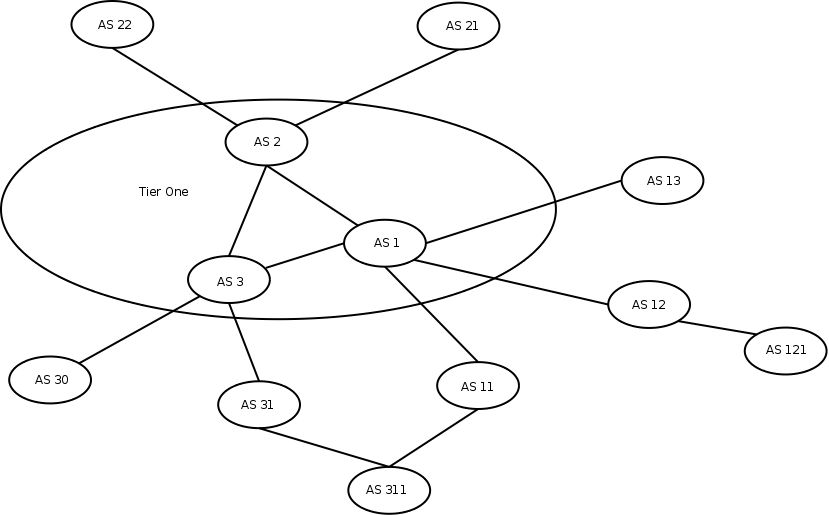
\includegraphics[width=16cm]{./schema/topologie_internet.png}
 }
  \caption{\label{topologie}Topologie d'Internet, exemple de repr\'esentation}
\end{figure}



%\end{document}


%\documentclass[a4paper,12pt]{article}


%\begin{document}

\subsection{Analyse de la topologie}

\par
Pour analyser la topologie de l'Internet \`a partir du graphe le repr\'esentant, nous disposons de plusieurs outils fournis par la th\'eorie des graphes.

\subsubsection{Les cliques}

Tout d'abord, la recherche des cliques permet d'identifier les endroits o\`u les AS sont tous reli\'es deux \`a deux, un de ces ensembles est constitu\'e des op\'erateurs du \textit{Tier One}. On retrouve aussi d'autres cliques localement.
%TODO peut etre a compléter

\subsubsection{La centralit\'e}

\par
Ensuite, comme il a été expliqu\'e lors de la pr\'esentation de la topologie de l'Internet, le graphe a une structure connexe, c'est-\`a-dire que si l'on prend deux sommets quelconques, il existe un chemin entre ces deux sommets.
Ce chemin passe par un certain nombre d'ar\^etes, et il est int\'eressant de savoir si telle ou telle ar\^ete est plus importante.
\par
Prenons l'exemple de deux AS A et B reli\'es entre eux. Nous savons qu'il existe une ar\^ete sur notre graphe entre A et B, supposons alors qu'il n'existe pas d'autres liens que celui entre A et B pour que les clients de A puissent joindre les clients de B. Ce lien revet donc une importance capitale puisque l'ensemble des routes partant des clients de A vers les clients de B passent par celui-ci.
\par
Il nous faut alors assigner des poids aux liens ou aux sommets afin de tenir compte de leur importance dans la structure globale.

\par
En th\'eorie des graphes, il existe un outil permettant d'\'evaluer l'importance des sommets ou des ar\^etes d'un graphe : la \textit{centralit\'e}. La centralit\'e permet de calculer le ratio du nombre de chemins passant par cette ar\^ete ou ce sommet par rapport au nombre de chemins total dans le graphe. Plus ce ratio est important plus le noeud ou l'ar\^ete est vital pour garder le caract\`ere connexe du graphe. La centralit\'e se calcule gr\^ace \`a la formule suivante :

\begin{figure}[!ht]
   \centering
   \frame
   {
      \parbox{12cm}
      {
         Soit un graphe G=(V,E) avec n sommets, la centralité $c_b(v)$ d'une arête v est :
         \begin{equation}
               c_b(v) = \sum_{\underset{s \neq v}s \neq v \neq t V} \frac{\sigma_st(v)}{\sigma_st}
         \end{equation}
	o\`u $\sigma_st$ est le nombre de plus court chemin allant de s vers t et $\sigma_st(v)$ est le nombre de plus court chemin de s vers t passant par v.
      }
   }
  \caption{\label{centralit\'e}Calcul de la centralit\'e}
\end{figure}



%\end{document}


% \documentclass[a4paper,10pt]{article}

% \begin{document}

\subsection{Repr\'esentation de la topologie}

Repr\'esenter Internet sous la forme d'un graphe peut s'av\'erer particulièrement difficile. En effet, si l'on regarde les donn\'ees r\'ecolt\'ees au niveau de diff\'erentes sources, on s'aperçoit que le graphe \`a repr\'esenter est immense : pour la topologie IPv4, il comporte plus de 40000 sommets et un nombre tout aussi cons\'equent d'ar\`etes.
\par
La topologie en IPv6 est \`a peine plus petite. Cela vient du fait que cette technologie n'est pas encore aussi largement r\'epandue que l'IPv4.

\par
Au tout d\'ebut du projet, nous avons essayé de repr\'esenter le graphe complet, avec tous ses sommets et toutes ses ar\^etes. Le r\'esultat obtenu \'est, comme on peut s'y attendre, confu et illisible. Il nous a donc fallu envisager des solutions pour all\'eger nos traitements et notre affichage.
\par
Voici une capture d\'ecran du programme lorsqu'il repr\'esente le graphe dans son int\'egralit\'e :
%TODO insérer ici une capture d'écran avbec le graphe complet
%TODO faire une figure et la référencer dans le paragraphe
\par
Le principe est de nettoyer le graphe en enlevant les AS feuilles qui sont tr\`es nombreux et pas nécessairement tr\`es pertinents pour une \'etude de la topologie du coeur de l'Internet. 
\par
%TODO Deplacer en partie IV, c'est l'élaboration du logiciel, contrairement à la partie 1 qui traite d'autre chose...
Dans un premier temps, on cible les AS qui n'ont ni client, ni PEER. Ce sont n\'ecessairement des feuilles, et par cons\'equent, nous pouvons les retirer du graphe pour faciliter sa lecture et alléger nos calculs.
\par Ensuite, notre tuteur de projet, Monsieur Meulle, nous a donn\'e un nouveau fichier, avec des relations entre AS sous la forme de triplets, permettant d'identifier tr\`es rapidement les AS feuilles.
Les liens entre AS sont plac\'ees sous la forme de triplets : {AS1, AS2, AS3} signifiant que ppour joindre l'AS3, l'AS1 a du passer par l'AS2. Ainsi, on peut identifier les AS de transit (ici l'AS2). Les AS feuilles sont alors facilement identifiables comme \'etant ceux qui ne jouent jamais le r\^ole d'As de transit dans les triplets.
%TODO Fin du déplacer...
\par
\'Etant donn\'e qu'Internet joue aujourd'hui un r\^ole important dans notre vie de tous les jours, tant au niveau professionnel que priv\'e, plusieurs \'etudes ont d\'ej\`a \'et\'e men\'ees pour mieux en comprendre la structure.
On trouve ainsi plusieurs ouvrage dans la litt\'erature et sur le net qui parle de ce sujet. On peut aussi trouver divers repr\'esentation graphique de l'Internet.
%TODO on pourrait ajouter cette image avec un commentaire, elle est sympa : http://en.wikipedia.org/wiki/File:Internet_map_1024.jpg

%\end{document}

\end{document}
